\section{Experiments}

\begin{figure}[ht]
\centering
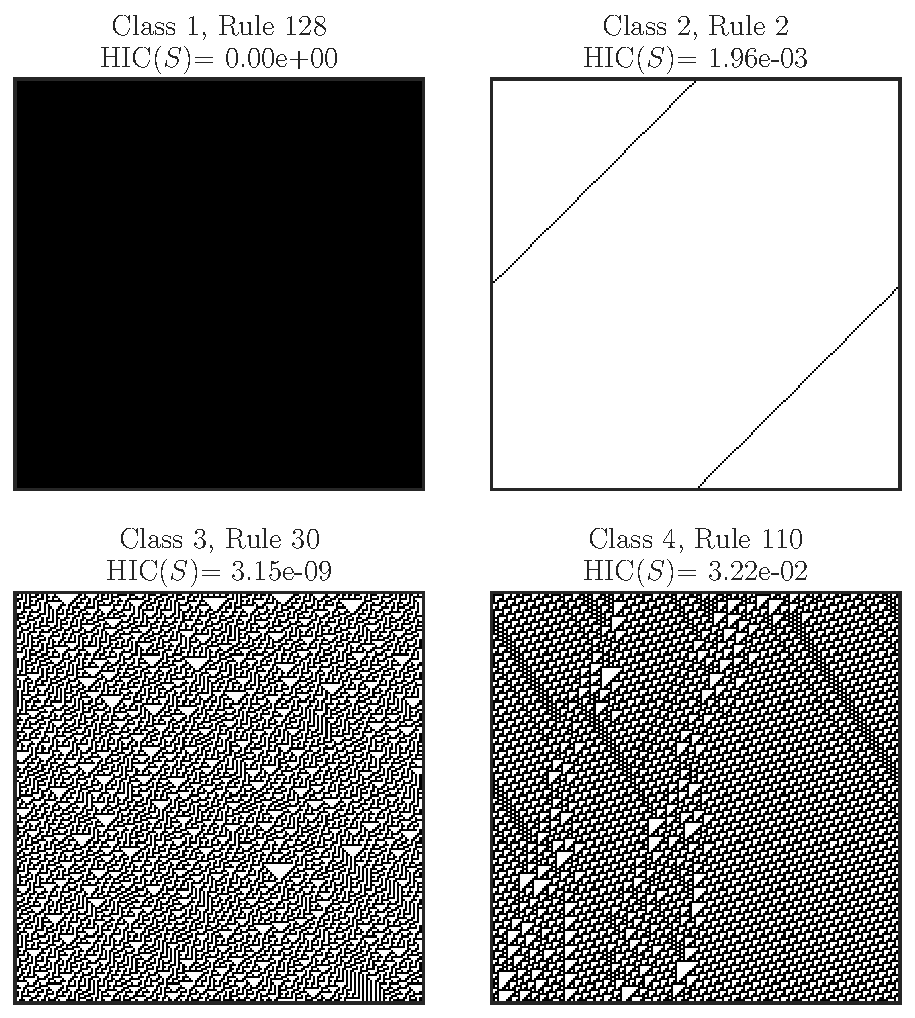
\includegraphics[width=0.7\textwidth]{figures/eca_images_and_hic}
\caption{TODO}
\label{fig:eca_images_and_hic}
\end{figure}

We examine HIC empirically using elementary cellular automata (ECA). Cells in
an ECA can take on one of two states. The update rule for a given state depends
on the state at the previous time step along with its two neighbors. Hence
there are $2^8 = 256$ possible ECAs. \citet{wolfram1983} proposed a four class
system to categorize ECA rules by their typical behavior. Class 1 ECAs converge
to a constant state, class 2 ECAs tend to exhibit periodic oscillations, class
3 ECAs show random behavior, and class 4 ECAs show complex behavior.

% TODO increase font size on figures
\begin{figure}[ht]
\centering
\begin{subfigure}{0.45\textwidth}
  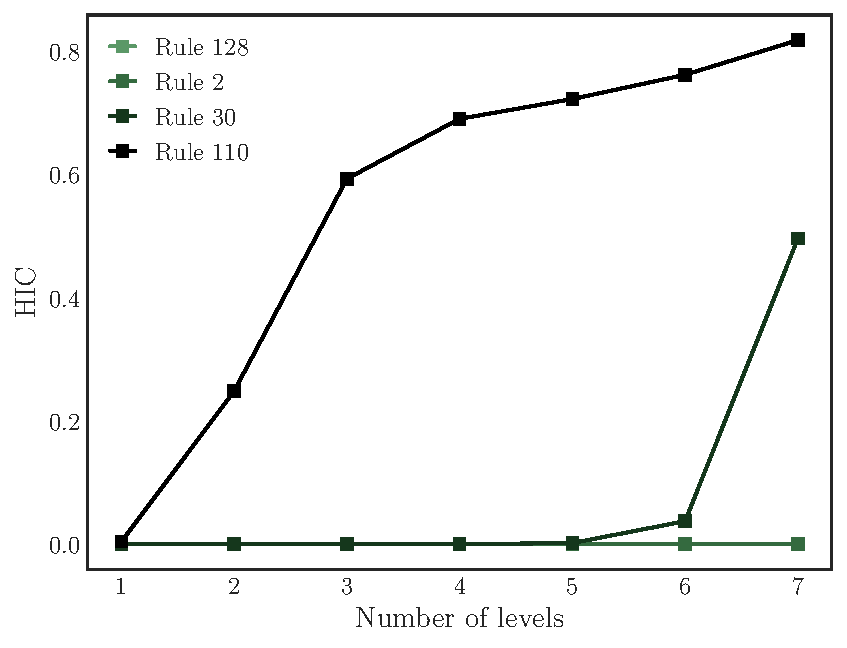
\includegraphics[width=1.0\textwidth]{figures/hic_vs_num_levels_size_200}
  \caption{$200 \times 200$}
\end{subfigure}
\begin{subfigure}{0.45\textwidth}
  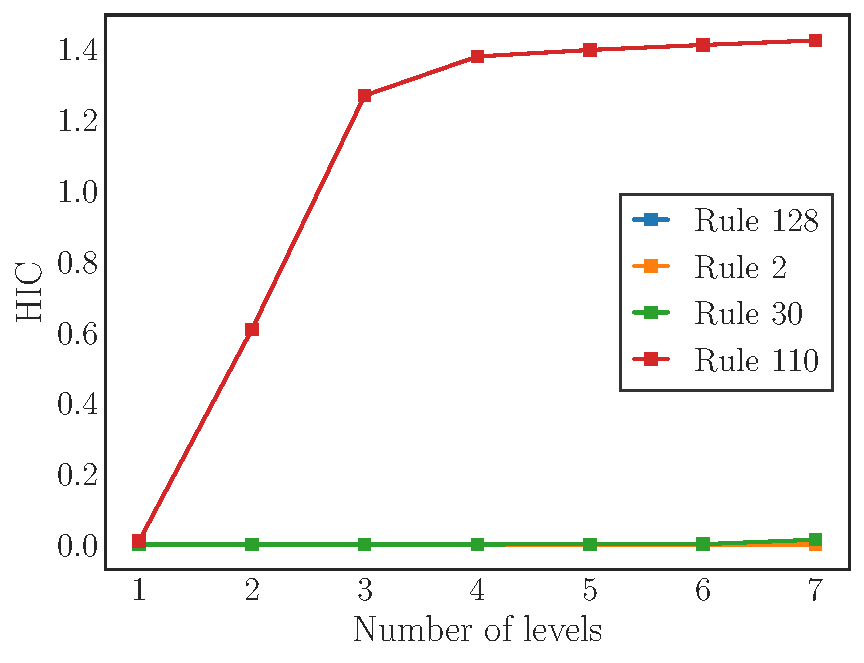
\includegraphics[width=1.0\textwidth]{figures/hic_vs_num_levels_size_500}
  \caption{$500 \times 500$}
\end{subfigure}
\caption{TODO}
\label{fig:hic_vs_levels}
\end{figure}


